\documentclass[]{politex}

% ========== Packages ==========
\usepackage[utf8]{inputenc}
\usepackage{amsmath,amsthm,amsfonts,amssymb}
\usepackage{graphicx,cite,enumerate}
\usepackage{subfiles}
\usepackage{caption}
\usepackage{pdfpages}
\usepackage{adjustbox}
\usepackage{wrapfig,lipsum}
\usepackage{verbatim}
\usepackage{listings}

% ========== Language options ==========
\usepackage[brazil]{babel}

% ========== ABNT (requer ABNTeX 2) ==========
%	http://www.ctan.org/tex-archive/macros/latex/contrib/abntex2
\usepackage[num]{abntex2cite}

% ========== Lorem ipsum ==========
\usepackage{blindtext}

% ========== Opções do documento ==========
% Título
\titulo{Robô Hospitalar: Hardware e Software}

% Autor
\autor{Vanderson da Silva dos Santos}

% Orientador / Coorientador
\orientador{Leopoldo Rideki Yoshioka}
%\coorientador{Nome do coorientador (opcional)}

% Tipo de documento
\tcc{}
%\dissertacao{Engenharia Elétrica}
%\teseDOC{Engenharia Elétrica}
%\teseLD
%\memorialLD

% Departamento e área de concentração
\departamento{Engenharia de Sistemas Eletrônicos}
\areaConcentracao{Engenharia de Sistemas Eletrônicos}

% Local
\local{São Paulo}

% Ano
\data{2021}

\begin{document}
% ========== Capa e folhas de rosto ==========
\capa
\falsafolhaderosto
\folhaderosto

%========== Folha de assinaturas (opcional) ==========
%\begin{folhadeaprovacao}
	\assinatura{Prof. Dr. Leopoldo Rideki Yoshioka}
%	\assinatura{Prof.\ Y}
%	\assinatura{Prof.\ Z}
%\end{folhadeaprovacao}

% ========== Ficha catalográfica ==========
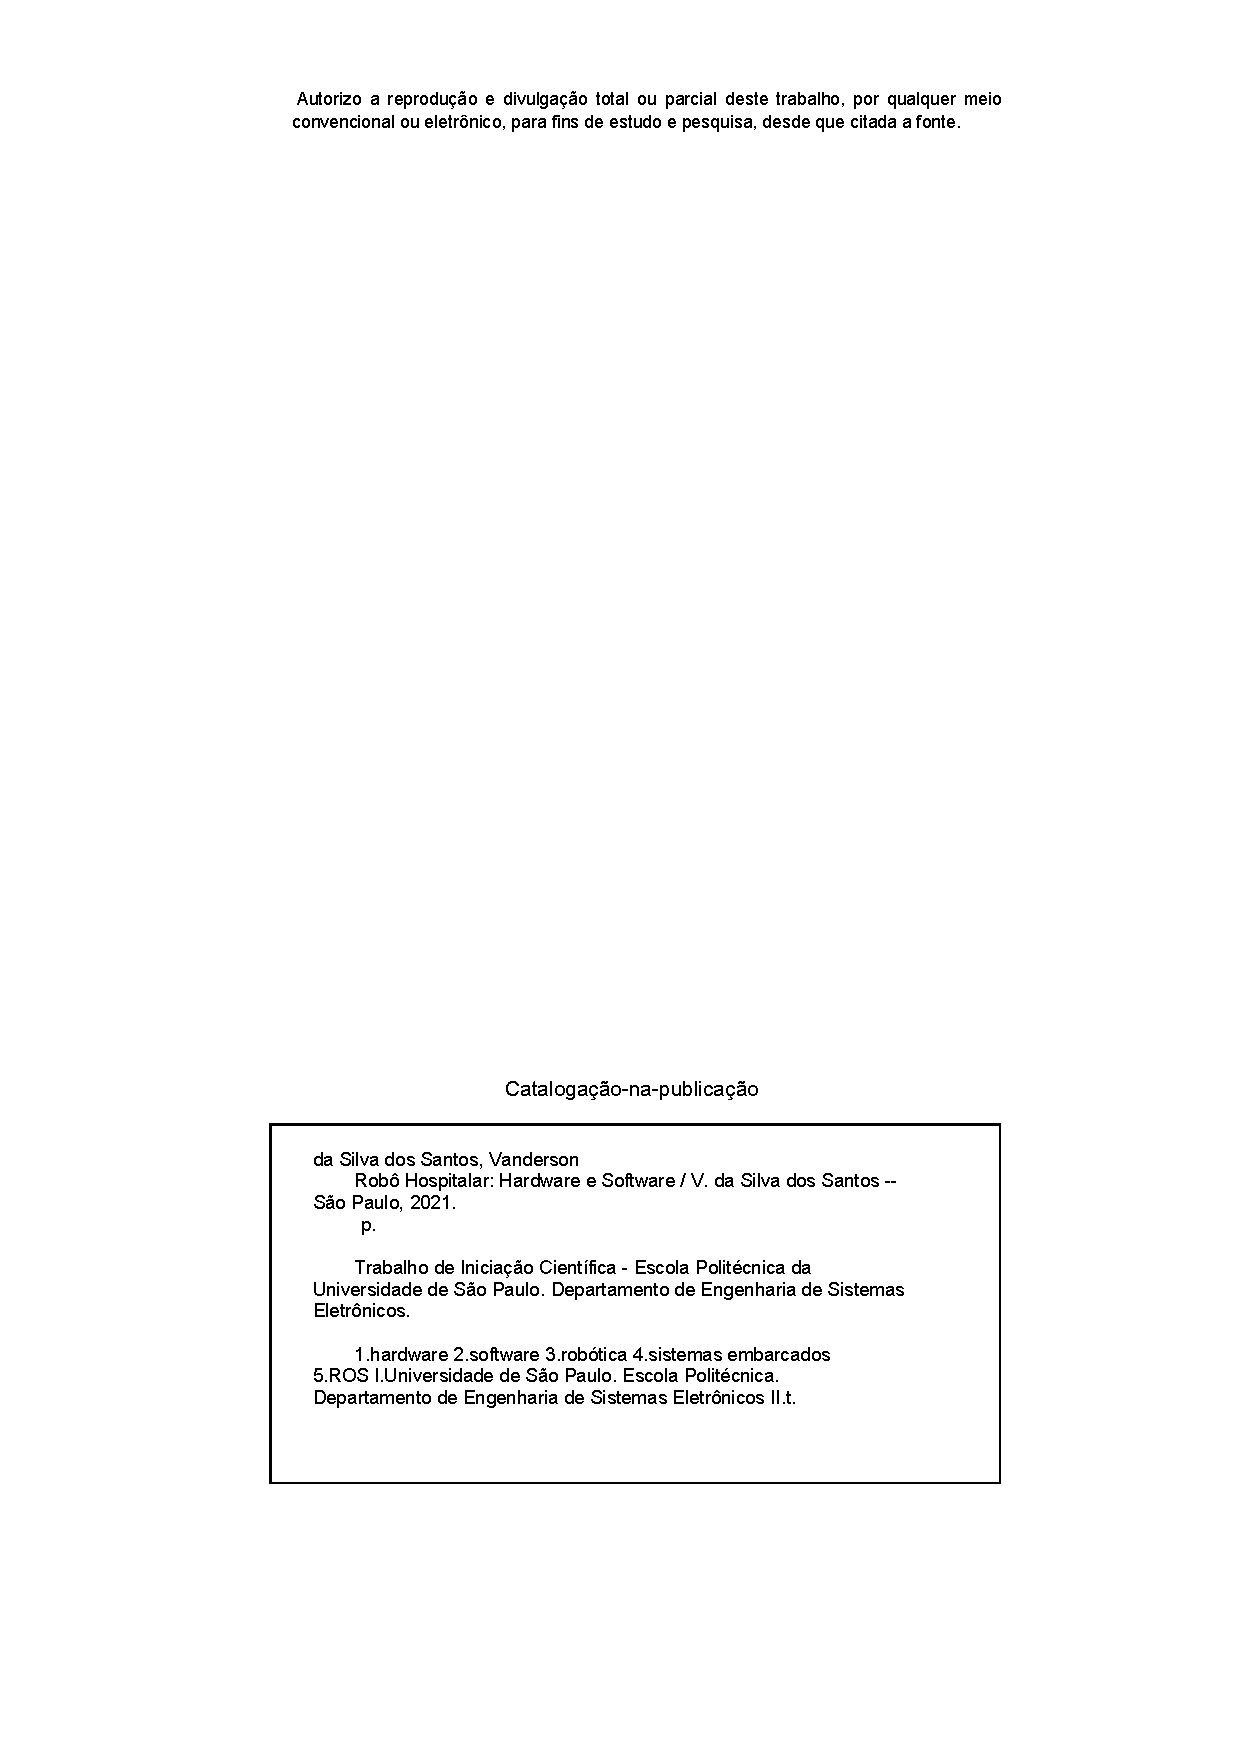
\includepdf{ficha_catalografica.pdf}

% ========== Dedicatória (opcional) ==========
\dedicatoria{Dedico esse trabalho aos amigos do Robô Hospitalar}

% ========== Agradecimentos ==========
\begin{agradecimentos}

Primeiramente, à minha família, que me deram suporte para ir e vir periodicamente na USP em um momento que transporte público não era aconselhado.

Ao meu professor orientador, Leopoldo Yoshioka, pela a oportunidade de participar do grupo , fazer a manutenção do projeto e sempre dar suporte, tanto em ajuda, quanto em ensinamentos .

Aos amigos do Robô Hospitalar, principalmente ao Lucas Boccia e Thomas Furukawa, que assume e vem assumindo uma postura administrativa, respectivamente, na equipe e ao Bruno Camara e o Pedro Croso, pelas noites de projetos e suporte. 

Aos amigos da equipe de robótica Thunderatz, que além de me presentear com uma base teórica e prática incrível, ainda estão sempre disponíveis para me dar suporte.


\end{agradecimentos}

% ========== Epígrafe (opcional) ==========
\epigrafe{%
	\emph{``Mas nunca imaginaria que a curiosidade fosse outra dessas tantas ciladas do amor''}
	\begin{flushright}
		- Gabriel Garcia Marquez
	\end{flushright}
}

% ========== Resumo ==========
\begin{resumo}
Toda a indústria de automação mundial, vem crescendo todo anos e como consequência contribuindo para um mundo mais eficiente. No âmbito da saúde, para corroborar para um atendimento ao paciente e garantir que os profissionais da realizem menos trabalhos repetitivos, diversos equipamentos vêm sendo desenvolvidos, dentre eles, robôs hospitalares. O objetivo deste trabalho é ,a partir desses princípios, a produção de um robô hospitalar que visa transportar medicamentos por todo um andar de um hospital. No âmbito do hardware,a proposta é fazer uma série de módulos eletrônicos embarcados que visam controlar e fazer manutenção do robô e reguladores de tensão, que garantam energia estável para os equipamentos eletrônicos. Por fim, no ponto de vista do Software, é desenvolver os algoritmos de controle com auxílio do framework ROS, realizar a simulação desses dados por Gazebo e Rviz e por fim, garantir todo o transporte dos dados pelo robô de maneira segura e confiável.
%
\\[3\baselineskip]
%
\textbf{Palavras-Chave} -- Autonomação, Algoritmos de Controle, ROS, Programação de Embarcados, Robótica.
\end{resumo}

\begin{comment}

% ========== Abstract ==========
\begin{abstract}
Abstract...
%
\\[3\baselineskip]
%
\textbf{Keywords} -- Word, Word, Word, Word, Word.
\end{abstract}
\end{comment}
% ========== Listas (opcional) ==========
\listadefiguras
\listadetabelas

% ========== Sumário ==========
\sumario

% ========== Elementos textuais ==========

% ========== Parte 1: Introdução ==========
\part{Introdução}
\subfile{chapters/introducao}

\subfile{chapters/objetivo}

\subfile{chapters/motivacao}

\subfile{chapters/metodologia}

\subfile{chapters/arquitetura_do_projeto}

% ========== Parte 2: Hardware ==========
\part{Hardware}

\subfile{chapters/distribuicao_de_energia}

\subfile{chapters/modulos_embarcados}

% ========== Parte 3: Software ==========
\part{Software}

\subfile{chapters/ambiente_de_simulacao}

\subfile{chapters/algoritmos_de_controle}

\subfile{chapters/integracao_software_hardware}

\begin{comment} % se sobrar tempo comentar


\subfile{chapters/desenvolvimento_web_mobile}
\end{comment}

% ========== Parte 4: Software ==========
\part{Resultados}

No âmbito da computação e da eletrônica, o software e hardware, que andam muito próximos um do outro, os resultados foram satisfatórios, mas nada além disso. Foi bastante trabalho em pouco tempo, porém, não foram realizados tantos testes quanto foi idealizado por conta de períodos sem poder frequentar a USP.

No que diz respeito ao Hardware, os módulos oficiais ainda não foram fabricados, pois é necessário revisar melhor os esquemáticos e testar todos os protótipos por completo para mandar fazer. Porém, levando em consideração que quase toda a reestruturação do projeto tem pouco menos de 8 meses, e poucos mais de 10 placas de circuito impresso foram sintetizadas, ainda é um bom resultado.

No que diz respeito ao Software, em pouco menos de 6 meses, todo o ambiente de simulação e algoritmos de controle foram produzidos. Por mais que o código da primeira versão fosse funcional, muito pouco era reaproveitável pela falta de organização e documentação de tudo desenvolvido. Por conta disso, tudo foi refeito. Contudo, tiveram-se muitos resultados produzidos e garantia de um código que pode ser repassado para futuras gerações de membros do projeto.


% ========== TITULOS DO SUMÁRIOS ==========
%\blinddocument
% =========================================

% ========== Referências ==========
% --- ABNT (requer ABNTeX 2) ---
%	http://www.ctan.org/tex-archive/macros/latex/contrib/abntex2
\bibliographystyle{abntex2-num}
\bibliography{bibliography}

% ========== Apêndices (opcional) ==========
\apendice
\subfile{chapters/visao_computacional}

% ========== Anexos (opcional) ==========
\anexo
\subfile{chapters/anexos}


\end{document}